\section{Approach} \label{sec:approach}
AdaPart-GNN addresses scalability and accuracy trade-offs in partition-based GNNs via three synergistic stages: (1) scale-adaptive partition determination, (2) Jaccard-eigenvector edge weighting, and (3) boundary prompt bridging (Figure~\ref{fig:approach}).

\textbf{1) Scale-Adaptive Partition Sizing ($K^*$):}
Fixed partition counts cause Out-Of-Memory (OOM) failures on massive graphs or severe community disruption on smaller graphs. To balance hardware limits with topological fidelity, we formulate a scale- and density-aware sizing heuristic:
{\setlength{\abovedisplayskip}{2pt}\setlength{\belowdisplayskip}{2pt}
\begin{equation} \label{eq:kstar}
K^* = \left\lceil \frac{|V|}{N_{\text{target}}} \cdot \left(1 + \beta \log_{10}\left(1 + \frac{2|E|}{|V|}\right)\right) \right\rceil
\end{equation}}
where $N_{\text{target}} \approx \frac{M_{\text{gpu}}}{\text{Mem}_{\text{node}}} \approx 35{,}000\text{--}40{,}000$ is the hardware-budgeted node capacity per subgraph ($\le 1.5$\,GB GPU allocation, accommodating feature tensors and SpMM buffers), setting $\frac{|V|}{N_{\text{target}}}$ as the baseline partition count. The average degree $\frac{2|E|}{|V|}$ measures structural density, penalizing edge-heavy graphs where message passing inflates activation memory, while $\log_{10}$ dampens power-law skews ($\beta \approx 0.35$). Intuitively, Equation~\eqref{eq:kstar} scales $K^*$ on massive graphs ($K^*=69$ on Products) to avoid OOMs while preserving relational structure on smaller graphs ($K^*=13$ on Arxiv).

\begin{figure}[t]
    \centering
    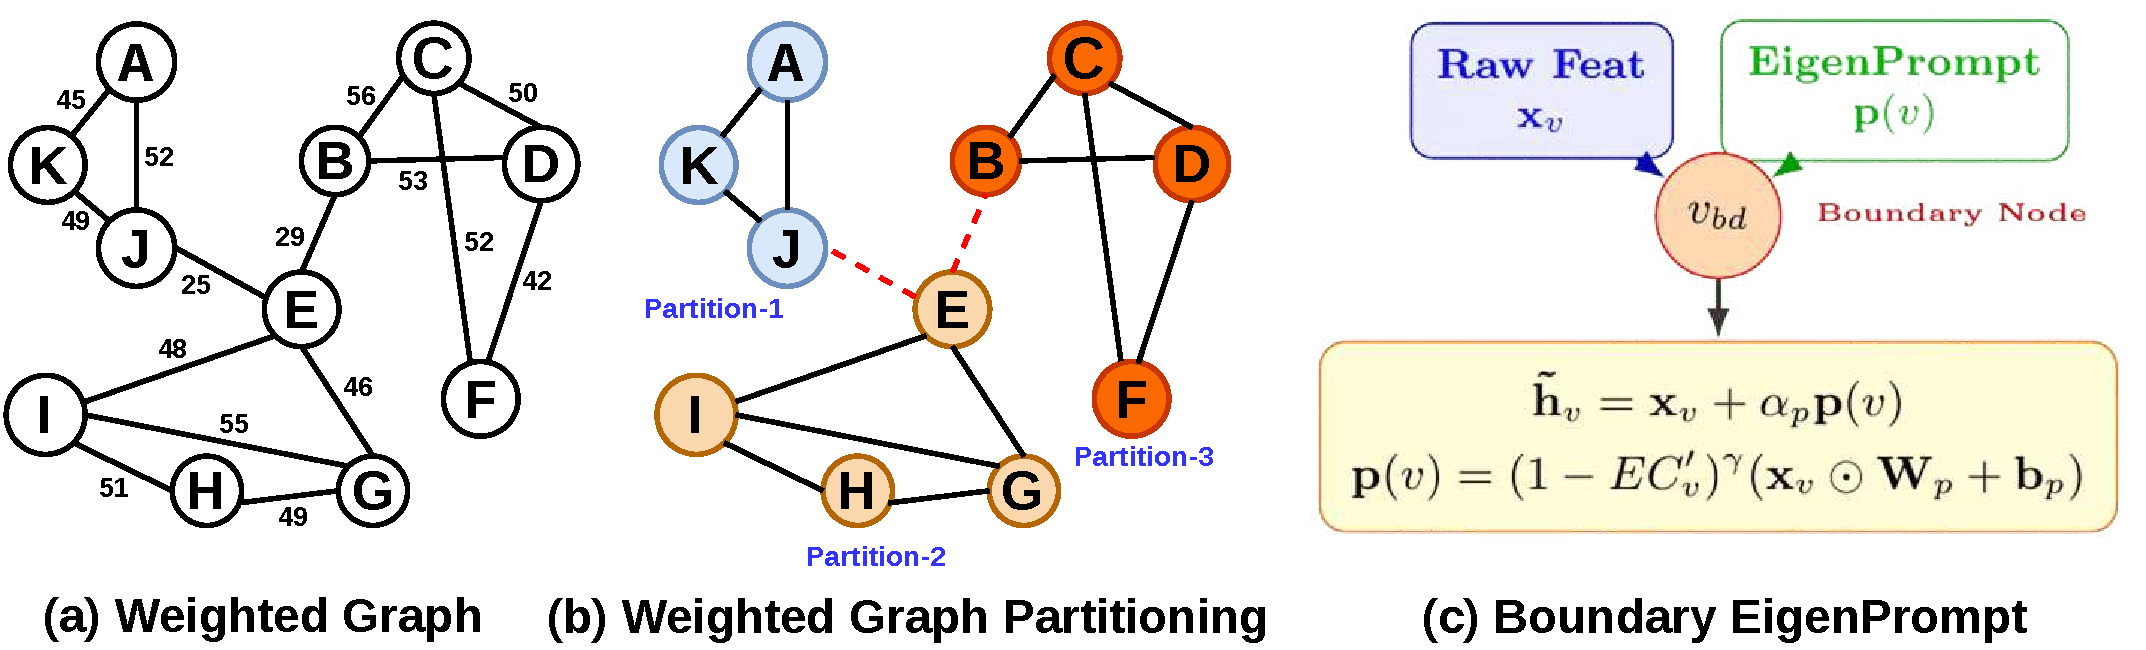
\includegraphics[width=0.98\columnwidth]{image/problem3_overview.pdf}
    \vskip 1mm
    \caption{AdaPart-GNN framework: (a) Weighted Graph, (b) Weighted Graph Partitioning with severed cuts, and (c) Boundary EigenPrompt bridging.}
    \label{fig:approach}
\end{figure}

\textbf{2) Jaccard-Eigenvector Edge Weighting:}
Standard METIS partitioning minimizes unweighted cuts, severing vital dense communities. To retain high-centrality pathways, we formulate a composite similarity combining neighborhood overlap (Jaccard) with global influence (eigenvector centrality):
{\setlength{\abovedisplayskip}{2pt}\setlength{\belowdisplayskip}{2pt}
\begin{equation} \label{eq:weight}
S_{uv} = J_{uv}^\alpha \cdot \left(\sqrt{EC'_u \cdot EC'_v}\right)^{1-\alpha}, \quad w_{uv} = 1 + \left\lfloor K_{\text{scale}} \cdot S_{uv} \right\rceil
\end{equation}}
where $J_{uv} = \frac{|N(u) \cap N(v)|}{|N(u) \cup N(v)|}$ captures community cohesion, and $EC'_v = \frac{EC_v}{\max_{k} EC_k} \in [0, 1]$ is the normalized eigenvector centrality. We empirically set $\alpha = 0.7$, balancing local cohesion with global topology while keeping $S_{uv} \in [0, 1]$. To satisfy METIS integer requirements, $w_{uv} = 1 + \text{round}(K_{\text{scale}} S_{uv})$ ($K_{\text{scale}} = 100$) maps weights to $[1, 101]$, guiding METIS to preserve cohesive partitions and cutting boundary loss by up to 8.1\% on Reddit.

% =========================================================================
% PREVIOUS VERSIONS (COMMENTED OUT FOR EASY RESTORATION IF NEEDED)
% =========================================================================
% \textbf{3) Boundary EigenPrompt Bridging:}
% Partitioning severs cross-partition edges during subgraph-batch training, starving boundary nodes $v \in \mathcal{V}_{bd}$ of global context. Cross-partition feature transfer incurs heavy communication latency. To compensate for lost global information with zero communication, we inject a Boundary EigenPrompt $\mathbf{p}(v)$ into node features $\mathbf{x}_v$:
% {\setlength{\abovedisplayskip}{2pt}\setlength{\belowdisplayskip}{2pt}
% \begin{equation} \label{eq:prompt}
% \mathbf{\tilde{h}}_v = \mathbf{x}_v + \alpha_p \cdot \mathbf{p}(v), \quad \mathbf{p}(v) = (1 - EC'_v)^\gamma \cdot (\mathbf{x}_v \odot \mathbf{W}_p + \mathbf{b}_p)
% \end{equation}}
% where learnable weights and biases $\mathbf{W}_p, \mathbf{b}_p \in \mathbb{R}^D$ are shared globally across all subgraphs to learn a global topological prior without inter-subgraph communication. The factor $(1 - EC'_v)^\gamma$ forms a topological boundary gate with empirically chosen $\gamma = 1.5$, providing super-linear suppression of prompt noise on semi-central nodes while fully activating on peripheral cut nodes ($EC'_v \approx 0$). For interior hubs ($EC'_v \approx 1$), the gate vanishes ($(1 - EC'_v)^\gamma \to 0$). With $\alpha_p$ scaling prompt strength and only $\mathcal{O}(D)$ parameters ($<6$\,MB overhead), this restores relational context with zero runtime communication.
% =========================================================================

\textbf{3) Boundary EigenPrompt Bridging:}
When a graph is partitioned, boundary nodes lose connections to neighbors in other partitions. While transferring cross-partition features restores this context, it causes heavy communication overhead. To solve this with zero communication, we inject a lightweight \textit{Boundary EigenPrompt} $\mathbf{p}(v)$ directly into node features $\mathbf{x}_v$:
{\setlength{\abovedisplayskip}{2pt}\setlength{\belowdisplayskip}{2pt}
\begin{equation} \label{eq:prompt}
\mathbf{\tilde{h}}_v = \mathbf{x}_v + \alpha_p \cdot \mathbf{p}(v), \quad \mathbf{p}(v) = (1 - EC'_v)^\gamma \cdot (\mathbf{x}_v \odot \mathbf{W}_p + \mathbf{b}_p)
\end{equation}}
Here, $\mathbf{W}_p, \mathbf{b}_p \in \mathbb{R}^D$ are learnable vectors shared across subgraphs to provide global context, and $\alpha_p$ is a scaling factor ensuring the prompt supplements rather than overpowers original node features $\mathbf{x}_v$. The term $(1 - EC'_v)^\gamma$ adaptively modulates prompt strength based on node centrality: isolated boundary nodes ($EC'_v \approx 0$) receive full prompt compensation, while well-connected interior hubs ($EC'_v \approx 1$) receive near-zero prompt ($(1 - EC'_v)^\gamma \to 0$) to protect intact features. Setting $\gamma = 1.5$ smoothly suppresses prompt noise on moderately connected nodes. Since only $\mathbf{W}_p$ and $\mathbf{b}_p$ are trained, the entire prompt module and its optimizer states consume $<6$\,MB of GPU memory, restoring boundary accuracy with zero runtime communication.
